\chapter{A Quick Overview of Other Tools}




%-------------------------------------------------------------------
%-------------------------------------------------------------------
%-------------------------------------------------------------------

\section{Developing raw and jpeg Images with Devlop}


%-------------------------------------------------------------------
%-------------------------------------------------------------------
%-------------------------------------------------------------------

\section{Making Ortho Mosaic with Porto}
\label{Porto}

\subsection{Introduction}

{\tt Porto}  is a tool for generating a complete mosaic from a set of \UNCLEAR{single}
ortho images generated by {\tt MicMac}. It is in a very basic state,
a lot of improvement would be required. By the way, I think  it can
still be useful for several applications.

To generate the tool:

\begin{center}
     make -f MakeOrtho
\end{center}

{\tt Porto} expects a parameter file like {\tt MicMac} and {\tt Apero}. It
must contain a structure {\tt CreateOrtho} as specified in {\tt SuperposImage.xml}.

The {\tt ExempleDoc/Boudha} data set contains an example of usage. Run it
by typing:

\begin{center}
                  bin/Porto ../micmac\_data/ExempleDoc/Boudha/ORTHO/Param-Porto.xml
\end{center}

   % - - - - - - - -  -- -  - - - - - - - -  - - - - - - - - - - - - - - - - - - - - - - - -

\subsection{Input to Porto}

The figure~\ref{Resul:Ortho:MM} presents the output of {\tt MicMac} that is used as
input to {\tt Porto}.
The input to {\tt Porto} consists of:

\begin{itemize}

   \item   a global meta-data  file specifying the geo-referencing of the
           DTM associated to the ortho;

  \item  a set of individual ortho-images;

  \item a set of mask images specifying for each ortho which images are visible;

  \item a set of incidence images, specifying the \UNCLEAR{priority};

  \item  a set of XML meta-data  associated to each image.
\end{itemize}


Figure~\ref{Indiv:Ortho} presents some individual ortho-images computed by MicMac on the
Buddha data set. The figure~\ref{Pb:Indiv:Ortho} presents some details of
the problems of each individual ortho-images. Figure~\ref{Incid:Ortho}
presents the incidence images.






\begin{figure}
\begin{tabular}{||c|c|c||}
   \hline \hline
   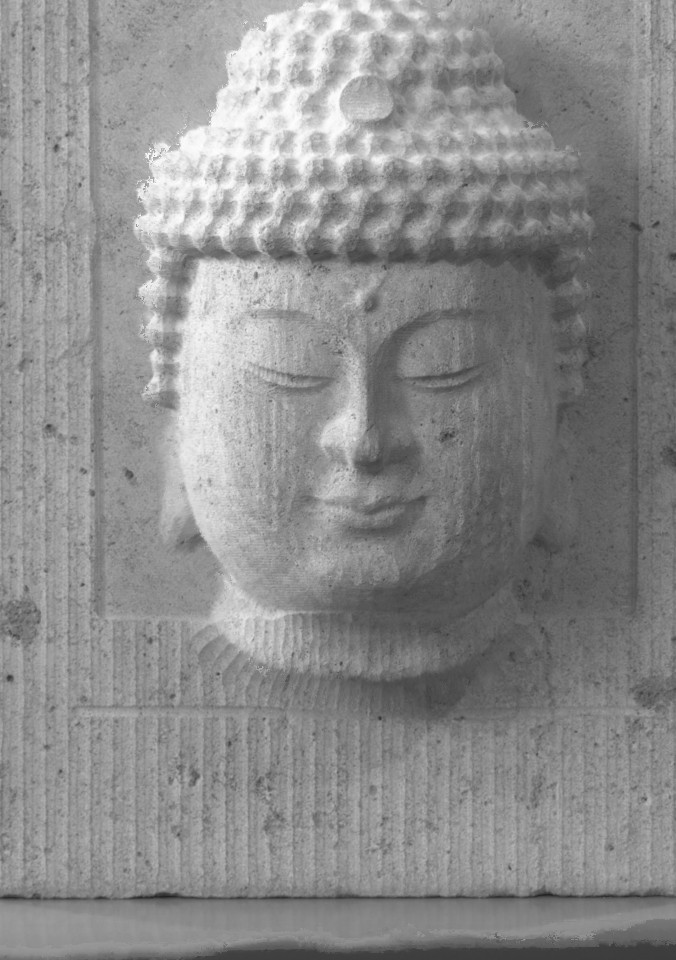
\includegraphics[width=55mm]{FIGS/Boudhas/Ort_IMG_5588.jpg}   &
   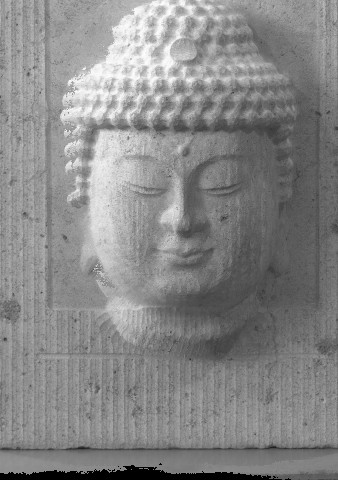
\includegraphics[width=55mm]{FIGS/Boudhas/Ort_IMG_5589.jpg}   &
   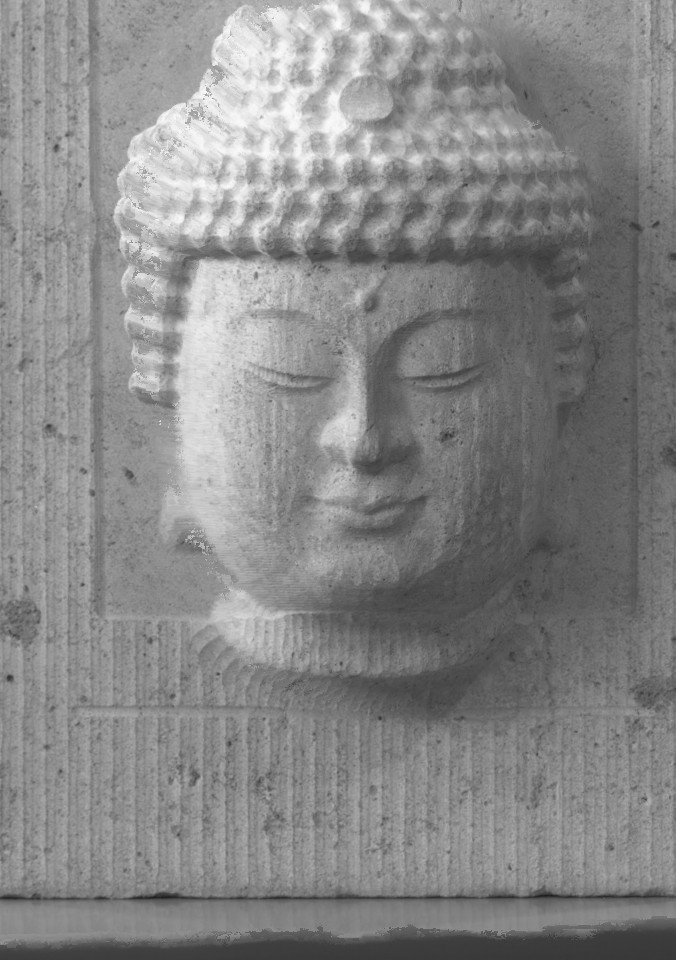
\includegraphics[width=55mm]{FIGS/Boudhas/Ort_IMG_5592.jpg}   \\ \hline  \hline
\end{tabular}
\label{Indiv:Ortho}
\caption{Three of the five individual ortho images}
\end{figure}



\begin{figure}
\begin{tabular}{||c|c||}
   \hline \hline
   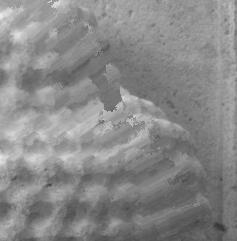
\includegraphics[width=80mm]{FIGS/Boudhas/PB-Ort_IMG_5591.jpg}   &
   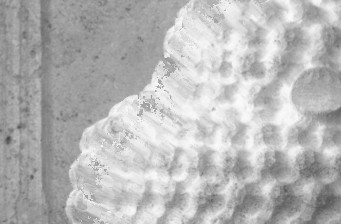
\includegraphics[width=80mm]{FIGS/Boudhas/PB-Ort_IMG_5592.jpg}   \\ \hline  \hline
\end{tabular}
\label{Pb:Indiv:Ortho}
\caption{Zoom on some problems of  individual ortho-image}
\end{figure}



\begin{figure}
\begin{tabular}{||c|c|c|c|c||}
   \hline \hline
   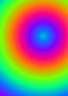
\includegraphics[width=30mm]{FIGS/Boudhas/Incid_IMG_5588_8Bits.jpg} &
   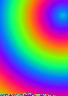
\includegraphics[width=30mm]{FIGS/Boudhas/Incid_IMG_5589_8Bits.jpg} &
   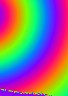
\includegraphics[width=30mm]{FIGS/Boudhas/Incid_IMG_5590_8Bits.jpg} &
   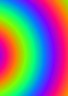
\includegraphics[width=30mm]{FIGS/Boudhas/Incid_IMG_5591_8Bits.jpg} &
   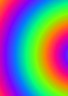
\includegraphics[width=30mm]{FIGS/Boudhas/Incid_IMG_5592_8Bits.jpg} \\ \hline  \hline
\end{tabular}
\label{Incid:Ortho}
\caption{ Incidence images computed for ortho priority}
\end{figure}

In the example {\tt Param-Porto.xml}, the section specifying these inputs is:


{\scriptsize
\begin{verbatim}
    <SectionEntree>
           <FileMNT> ../MEC-7-Ter/Z_Num5_DeZoom1_LeChantier.xml </FileMNT>
           <KeySetIm>  NKS-Set-OfPattern@Ort_(.*)\.tif </KeySetIm>
           <KeyAssocMetaData > NKS-Assoc-ChangPrefixAndExt@Ort_@tif@PC_@xml  </KeyAssocMetaData>
           <KeyAssocNamePC >   NKS-Assoc-ChangPrefixAndExt@Ort_@tif@PC_@tif </KeyAssocNamePC>
           <KeyAssocNameIncH>  NKS-Assoc-ChangPrefixAndExt@Ort_@tif@Incid_@tif </KeyAssocNameIncH>
    </SectionEntree>
\end{verbatim}
}

The {\tt <FileMNT>} is an XML-meta-data file containing information about the DTM produced
by {\tt MicMac}. Its tags have been described in~\ref{Ex:GrTer:RA}. The ortho-mosaic produced
by {\tt Porto} will have the same geo-referencing as the DTM. The other arguments are
keys for describing sets and associations. The functioning is quite classical now:

\begin{itemize}
    \item {\tt <KeySetIm>} describes the set of individual ortho images;
    \item {\tt <KeyAssocMetaData>} is a key for computing the name of XML-Meta data from the name of individual ortho image;
    \item {\tt <KeyAssocNamePC>} is a key for computing the name of the \UNCLEAR{hidden part image} from the name of individual ortho image;
    \item {\tt <KeyAssocNameIncH>} is a key for computing the name of the incidence image from the name of individual ortho image;

    \item \UNCLEAR{this is the same key}, that is used with different parameters; this key allows to change the
          beginning (prefix) of a name and its extension.

\end{itemize}

Here is {\tt PC\_IMG\_5588.xml}, an example of one of the meta-data file:


{\scriptsize
\begin{verbatim}
<MetaDataPartiesCachees>
     <Done>true</Done>
     <Offset>0 0</Offset>
     <Sz>676 960</Sz>
     <Pas>1</Pas>
     <SeuilUse>3</SeuilUse>
     <SsResolIncH>10</SsResolIncH>
</MetaDataPartiesCachees>
\end{verbatim}
}

The important tags are:

\begin{itemize}
   \item {\tt <Offset>} and {\tt <Sz>} specify the position of the individual ortho-photo
         on the DTM. Because, of course, in real example, the individual ortho-photo  will be much smaller
         than the DTM or resulting mosaic, so it will be stored only a sub-rectangle of the global DTM;

   \item {\tt <SeuilUse>} is a real value, use \UNCLEAR{to threshold} the  images ({\tt PC\_IMG\_5588.tif} \dots) and
         defining which pixel must be used;

   \item {\tt <SsResolIncH>} is the resolution of incidence images ({\tt Incid\_IMG\_5588.tif} \dots)
         in fact as these images are very regular, it would be useless to store them at full resolution.

\end{itemize}


As this file have been generated automatically by {\tt MicMac}, in most cases you will
not need to modify it, but it is still good to understand a bit how things work,
in case of problems \dots


   % - - - - - - - -  -- -  - - - - - - - -  - - - - - - - - - - - - - - - - - - - - - - - -

\subsection{Output to Porto}

Once  all these inputs are \UNCLEAR{known}, %nom ou adjectif?
the mosaicing
algorithm is quite obvious:

\begin{itemize}
     \item for each pixel of  the output image:
     \begin{itemize}
          \item select the unmasked image having the lowest incidence.
     \end{itemize}
\end{itemize}

The parameters specifying the output are:

{\scriptsize
\begin{verbatim}
     <SectionSorties>
           <SzDalle>    1000            </SzDalle>
           <SzBrd>      100             </SzBrd>
           <NameOrtho>  Ortho-NonEg-Test-Redr.tif </NameOrtho>
           <NameLabels>  Label-Test-Redr.tif</NameLabels>
     </SectionSorties>
\end{verbatim}
}

{\tt NameOrtho} specifies the name of the ortho mosaic. {\tt NameLabels} is an optional
argument, when specified, {\tt Porto} creates a label image indicating for each pixel which
individual  image is to be used for \UNCLEAR{filling the geometry}.  \UNCLEAR{Figure~\ref{Resul:Ortho}} %pas bon le nr de la fig
presents the main results.


\begin{figure}
\begin{tabular}{||c|c||}
   \hline \hline
   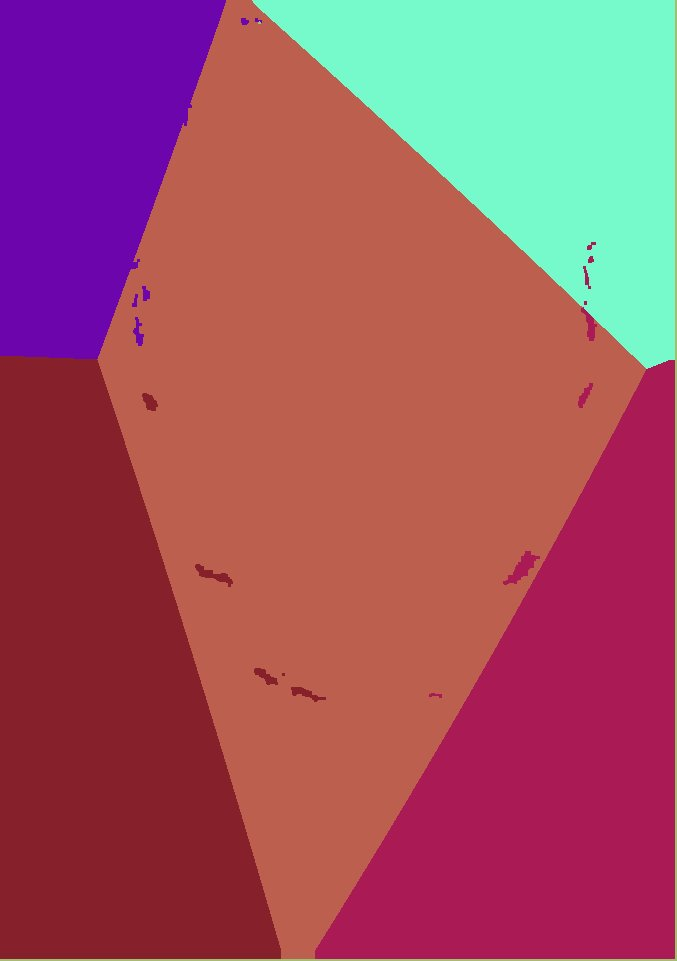
\includegraphics[width=80mm]{FIGS/Boudhas/Label-Test-Redr.jpg}   &
   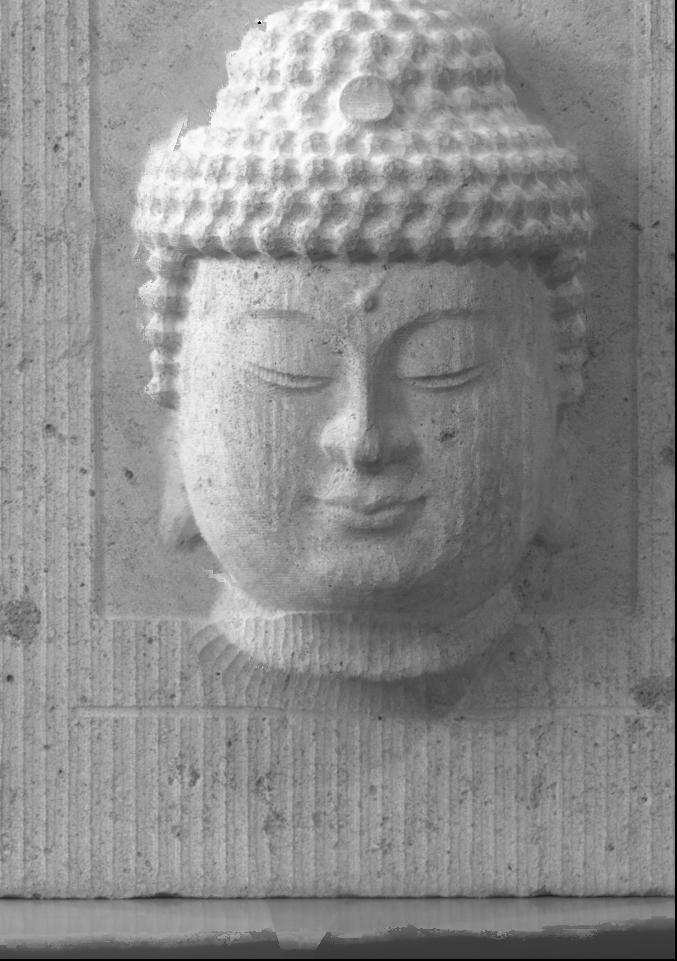
\includegraphics[width=80mm]{FIGS/Boudhas/Ortho-NonEg-Test-Redr.jpg}   \\ \hline  \hline
\end{tabular}
\label{Resul:Ortho}
\caption{Computed label images and resulting ortho images}
\end{figure}



   % - - - - - - - -  -- -  - - - - - - - -  - - - - - - - - - - - - - - - - - - - - - - - -

\section{V.O.D.K.A.}
\label{V.O.D.K.A.}

\subsection{Theory}

The vignetting is an optical effect that results in a gradual radial drop-off in images (the corners of images are relatively darker than the center). The figure (\ref{image_vignette}) shows an example of this effect.

\begin{figure}[htb]
\centering
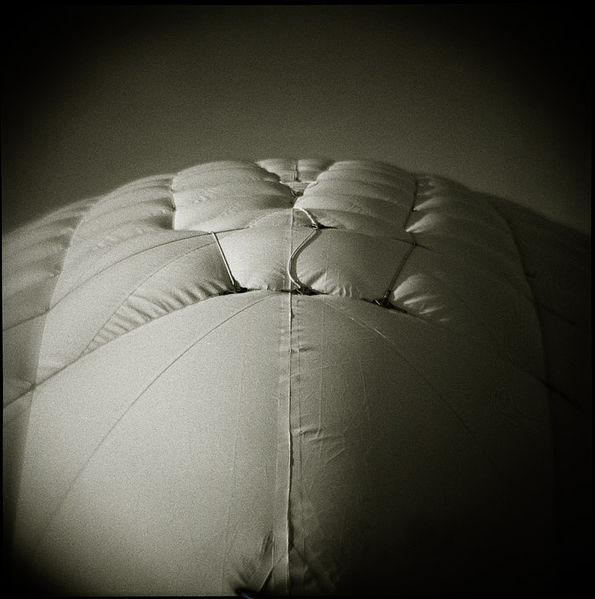
\includegraphics[width=6cm]{FIGS/Arsenic/595px-Swanson_tennis_center.jpg}
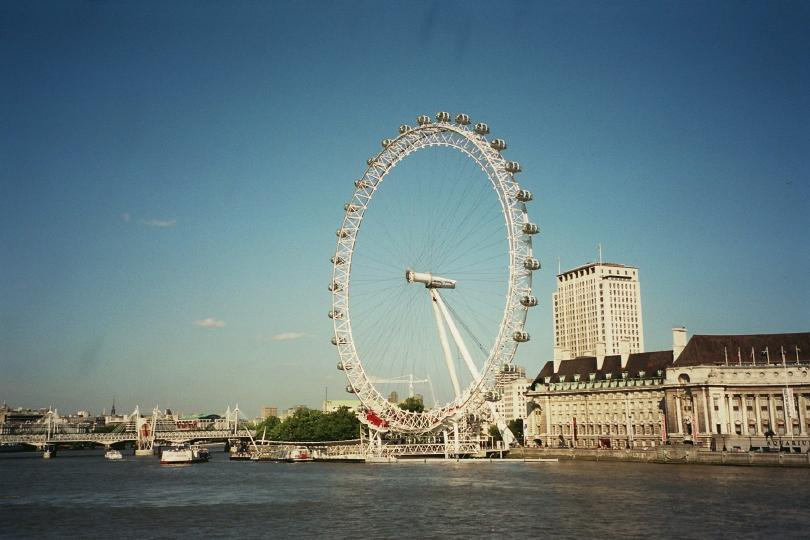
\includegraphics[width=6cm]{FIGS/Arsenic/London_eye_501588_fh000038.jpg}
\caption{
Different vignetting effect
%Vignette from the Nikkor 18-105 mm VR, F/3.6,18mm, fixed on a Nikon D90. The image is one of an homogeneous grey field
}
\label{image_vignette}
\end{figure}

Read more about vignetting :
\begin{itemize}
   \item \url{http://en.wikipedia.org/wiki/Vignetting}
   \item \url{http://fr.wikipedia.org/wiki/Vignettage}
\end{itemize}

\subsection{Name and function}
Vodka stands for "\textit{Vignette Of Digital Kamera Analysis}".

This command estimates the vignetting effect for a set of images with the same aperture and focal length without the need of a laboratory setup (classically an integrating sphere). The vignette model that is used is an even 6th degree polynomial function centered on the middle of the image. With r the distance to the center of the image and $\alpha$, $\beta$ and $\gamma$ the polynomial coefficients, we have : \[V(r)=1+ \alpha r^2 + \beta r^4 + \gamma r^6\]


The computation of the model uses a RANSAC based algorithm to solve the sets of equation of the following type (where $G_{i}$ is the grey value of a tie point for the image i and r the distance to the center of the image) : \[ G_{1}-G_{2}=\alpha(G_{2}*r_{2}^2-G_{1}*r_{1}^2)+\beta(G_{2}*r_{2}^4-G_{1}*r_{1}^4)+\gamma(G_{2}*r_{2}^6-G_{1}*r_{1}^6) \]

Between 9 and 30 points are randomly selected from the tie points and a solution is computed using least square matching. The solution is then awarded a score : \[Score=\frac{P_{inliers}}{EMP}\].

Where:
\begin{itemize}
\item \textit{$P_{inliers}$} the percentage of the tie points complying with the model ($\pm 2\%$) $\Rightarrow$ for good models, a value about 20\% to 40\% is expected.

\item \textit{EMP} the mean error between the model and the points weighted by $min(r_{1},r_{2})$ to increase the importance of points away from the image center (and therefor more influenced by vignetting).
\end{itemize}


\subsection{Input data}
To use this command, a set of images with the same aperture and focal length, taken in a stable illumination setting is necessary. The command also requires the computation of tie points (through Tapioca).


Calling the command is done with the following command line (where ImagesPattern is the regular expression describing the set of images ) : \[mm3d\;Vodka\;ImagesPattern\]

Multiple datasets can be processed at once, the program would then sort the images in subsets with the same aperture and focal length and give a solution for each subset.

\subsection{Output data}
For each aperture/focal length combination in the input set, the commands create a floating point .tif file of the image's size named Vignette/Foc0000Dia111.tif, where 0000 is the focal length in millimeters and 111 the aperture times 10.


Corrected images can also be created if asked by the user, mostly for quality checking (see bellow).


\subsection{Options}
\begin{itemize}
\item{\textit{DoCor (bool)} toggle the creation of corrected images (Def=false)}
\item{\textit{InCal (string)} Name of folder with vignette calibration tif file (if previously computed)}
\item{\textit{InTxt (string)} True if homologous points have been exported in txt (Def=false)}
\item{\textit{Out (string)} Output folder (Default=Vignette)}
\end{itemize}

\subsection{How to use VODKA}
Vodka is to be used to compute a vignette calibration. The best results are obtained with images where tie points are at different distances from the image center in the images that generated them, typically non-convergent images.


The output files should then be placed in a folder with other images taken with the same camera and the same aperture/focal length combination. The images that will be created in the Tmp-MM-Dir (and therefor used by every other commands) when the proper VODKA output files are present will be corrected using those files. If you want to use the VODKA results on the images used to compute it, you should place the VODKA output files in the images' directory and delete the Tmp-MM-Dir folder.

\section{A.R.S.E.N.I.C}
\label{A.R.S.E.N.I.C.}
\subsection{Name and function}
ARSENIC stands for \textit{Automated Radiometric Shift Equalization and Normalization for Inter-image Correction}.


This function corrects the key images used for coloring point clouds in order to have a smooth transition between sub-clouds of the same scene. It is designed to be used with the "GeomImage" correlation geometry.


\textcolor{red}{ This function is not designed for the equalization of images prior to image mosaicing}

\subsection{Input data}
\label{inputArsenic}

ARSENIC require a depth map for each image that will be equalized, computed with MICMAC/Malt. The dense radiometric tie point algorithm used in this program requires very well co-registered depth maps (or point clouds).
Calling the command is done with the following command line (where ImagesPattern is the regular expression describing the set of images ) :\[mm3d\;Arsenic\;ImagesPattern\]

\subsection{Output data}
The output of this command is the corrected images, by default in a folder called Arsenic. These images can then be used to color a point cloud through Nuage2Ply.

\subsection{Options}
\begin{itemize}
\item{\textit{TPA (Tie Point Accuracy - int)} defines the precision threshold for the tie points (def=16, means $\frac{1}{16}$ of pixel resolution)}
\item{\textit{ResolModel (int)} defines the resolution of the model to be used in the tie point computation (def=16 for DeZoom 16)}
\item{\textit{InVig (string)} defines a vignette calibration folder (if any)}
\item{\textit{Out (string)} defines the output directory}
\item{\textit{NbIte (string)} defines the number of iterations of the process (def=5)}
\item{\textit{ThreshDisp (string)} defines the disparity threshold between the tie points (Def=1.4 for 40\%)}
\end{itemize}

\subsection{Algorithm}

\subsubsection{Tie point detection}

In order to have a more accurate, denser and more interest-zone focused set of tie points, the tie points are extracted from the result of the dense correlation.


 Every point situated in the mask of a key image is projected in 3D through the depth map generated by MICMAC/Malt, then reprojected in the other key images and finally projected again in 3D if the second projection resulted in a point in the secondary key image's mask. If the two 3D projections result in a similar point (the concept of similarity being defined through the TPA option : the maximum distance between two 3D projections that validates the points being $PixelResolution/TPA$). For each validated point, the image coordinates of the point in the key image is recorded, as well as the factors $K$ between the pixel values of each images for all channels : \[K=(1+G_{j})/2*G_{i}\]
 With \textit{G} a grey value, \textit{i} the primary key image and \textit{j} the secondary image that generated the tie point. A tie point is therefor an object with 5 values, $Point=(X,Y,K_{R},K_{G},K_{B})$. The $+1$ is a call to the initial value.

\subsubsection{Equalization}

In a first step, a correction factor is computed for each tie point with an inverse distance weighting and a self weighting value (the image is self influencing). For each radiometric channel of each point, $j$, we have the following formula ($i$ is the tie point currently used in the interpolation):
\[Cor(TiePointj)=\sum_{i=1}^{n} \frac{(K_{i})/2}{\sqrt{(X_{i}-X_{j})^2+(Y_{i}-Y_{j})^2}}\]

This process is then iterated. A filtering system is yet to be developed to prevent radiometric outliers to push the model after too many iterations. An outlier is a point where Kr, Kg or Kb is more than \textit{ThreshDisp}\% different than the average value for the image considered.


The corrected tie points are then applied to a grid also through inverse distance weighting, the interpolated to the whole image through bilinear interpolation. The grid is computed by the formula bellow, with $i$ the tie point index and $(X,Y)$ the grid point's coordinates : \[Cor(X,Y)=\sum_{i=1}^{n} \frac{K_{i}}{\sqrt{(X_{i}-X)^2+(Y_{i}-Y)^2}}\]

\begin{figure}[H]
\centering
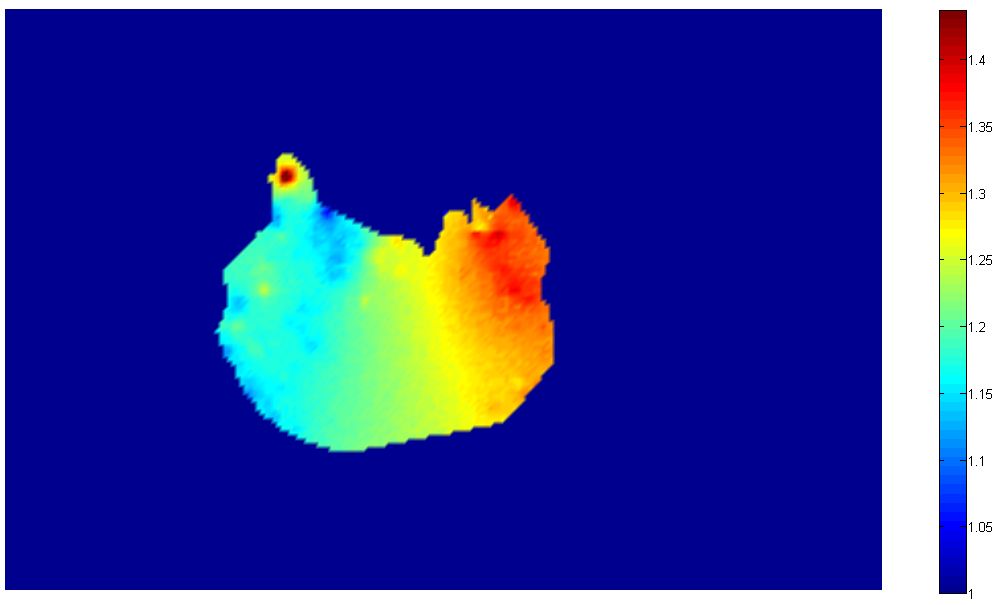
\includegraphics[width=15cm]{FIGS/Arsenic/SurfCorr.png}
\caption{Example of a correction surface}
\label{SurfCorr}
\end{figure}


\subsection{How to use ARSENIC}

Once the appropriate input data (see~\ref{inputArsenic}) is computed, the command can be run. The images produced in the output folder are to be used as "Attr" arguments in the "Nuage2Ply" command to produce equalized sub-point clouds.



